
\section{Higher-Order Dynamics in CISM}
\label{sc:higher-order-into}

\subsection{Basics}
The main distinction between so-called higher-order models and 0-order (or ``shallow ice") models is that higher-order models attempt a closer approximation to solving the nonlinear Stokes equations. This usually means incorporating some approximation of horizontal-stress gradients (along-flow stretching or compression and across-flow shearing) in addition to the vertical stress gradients that are accounted for in shallow ice models (Figure \ref{fig:stressbalance}). This is important for several reasons:

\begin{figure}
  \begin{center}
    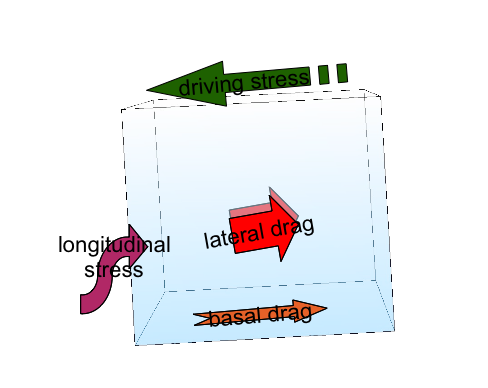
\includegraphics[width=0.5\columnwidth]{\dir/figs/StressBalance.eps}
  \end{center}
  \caption{The gravitational stress available to move the ice is the driving stress, indicated in green. Because the ice is assumed to be in equilibrium, the sum of the other stresses is equal to (i.e., must balance) the gravitational driving stress. In the 0-order model (shallow-ice approximation) the driving stress is assumed to be balanced by basal drag alone. In higher-order models, this restriction is relaxed and the balance of stresses now includes lateral and/or longitudinal stresses. Because these stresses must be computed based on conditions outside the local ice column, the model becomes significantly more complex.}
  \label{fig:stressbalance}
\end{figure} 

\begin{itemize}
\item For the ice-sheet regions of greatest interest -- e.g. ice streams, ice shelves, and other regions of fast flow -- horizontal-stress gradients are at least as important as vertical stress gradients. To model the flow accurately in these regions, higher-order models are required.

\item The shallow-ice approximation, applied to situations in which there is basal sliding, gives rise to a singularity in the vertical velocity. Models compute the vertical velocity by integrating the incompressibility equation:

\begin{equation}
  \label{ho.eq.incompress}
  \frac{\partial w}{\partial z} = -\frac{\partial u}{\partial x}-\frac{\partial v}{\partial y}.
\end{equation}

If there is a jump 
from no sliding in one grid cell to sliding in an adjacent cell, the horizontal velocity gradients at the bed will depend on the grid spacing; the horizontal gradients (and through incompressibility, the vertical velocity gradient and thus the vertical velocity) will become increasingly large as the grid spacing decreases. Obviously, this should be avoided.

\item Near the grounding line (the boundary between grounded and floating ice), horizontal rather than vertical stresses often control the flow. Incomplete knowledge of the stresses makes it unlikely that shallow ice models will ever be able to accurately simulate grounding-line advance and retreat.

\item In some regions of very slow flow, like ice divides, horizontal-stress gradients are important or dominant. Ice cores are often recovered at ice divides, and flow modeling is important for interpreting ice core records and using information (such as layer thickness) to infer the past flow history in the region. In order to model that flow correctly, one must include horizontal stresses. (At an ice divide the surface slope is \(\sim\)0, in which case vertical stress gradients that drive deformation in 0-order models are also \(\sim\)0. In reality, deformation is not 0 at ice divides, but is controlled by horizontal stretching rather than vertical shearing).
\end{itemize}

The term ``higher-order'' comes from scaling analyses of the Stokes equations for which a scaling parameter $\lambda=H/L$ (the ratio of the thickness to the horizontal length scale of interest) is used to assign importance to the various terms. Shallow ice models retain only terms of order 0 while higher-order models also retain terms of order 1 (and possibly more) (Figure \ref{fig:hoeqns}). 

\begin{figure}
  \begin{center}
    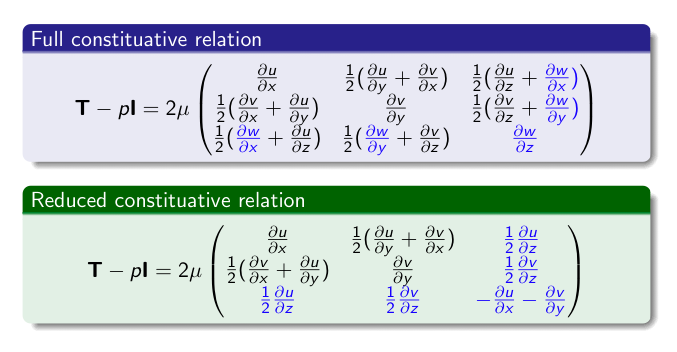
\includegraphics[width=0.7\columnwidth]{\dir/figs/HOeqns.eps}
   \end{center}
  \caption{Stokes-flow (top) and first-order (bottom) constitutive equations, which relate stresses to strain rates (and in turn to velocity gradients). \textbf{$\tau$} is the deviatoric stress tensor, \textit{\textbf{I}} is the identity tensor, \textit{P} is the pressure, and $\eta$ is the effective ice viscosity. The strain rate tensor is given by the term in parentheses on the right-hand side of the equation. For the first-order approximation (bottom), the bold terms from the Stokes equations are assumed negligible.}
  \label{fig:hoeqns}
\end{figure} 

\subsection{Available schemes}

\begin{itemize}
\item The most fundamental higher-order scheme is the full set of nonlinear Stokes equations. Because of the computational burden, many large-scale 3D models solve lower-order approximations of the Stokes equations (Figure \ref{fig:phylogeny}). However, several groups have made significant advances in Stokes modeling
(e.g. the ELMER-Ice effort; \citet{gagliardini:2013iv}). 
Current DOE-funded efforts include implementation of a nonlinear Stokes model on unstructured grids \citep{Leng:2012ia}.
\end{itemize}

\begin{itemize}
\item 
Probably the most long-lived higher-order approximation in glaciology is the shallow-shelf approximation (or SSA) describing flow within an ice shelf. While not truly ``higher-order" when only applied to ice shelf flow, it can provide nearly equivalent results to ``true" higher-order models in cases where basal drag is small but non-zero (e.g., for modeling the flow of ice streams). The SSA was developed and made popular by Douglas MacAyeal (e.g., \citet{Macayeal:1989uo}). 
Its main disadvantage is that it is not fully 3D, as it assumes uniform velocity throughout the ice thickness driven only by horizontal stress gradients. It is adequate for describing fast flow in many parts of ice sheets, such as ice shelves and some ice streams. In these regions, not resolving vertical gradients is a computational advantage.   
\end{itemize}

\begin{itemize}
\item The SSA equations are actually a depth-averaged form of a more general higher-order model, commonly referred to as the ``Blatter-Pattyn model" (\citet{BLATTER:1995wz}; \citet{Pattyn:2003tj}). 
Blatter-Pattyn dynamics, synonymous with and more formally described as the ``first-order accurate Stokes approximation"\footnote{See \citet{Schoof:2010dl} and \citet{DUKOWICZ:2010wb} for a more complete scaling analysis and derivation of the first-order Stokes approximation.}, are implemented in CISM's default higher-order dynamical core, Glissade.
\end{itemize}

\begin{itemize}
\item Another formally first-order accurate Stokes approximation, which might be considered ``quasi" three-dimensional, is the so-called ``L1L2" approximation \citep{Schoof:2010dl}. This model combines a two-dimensional SSA solve and a one-dimensional (column) SIA solve in a mathematically rigorous way. The model solution, from a combination of SSA (for approximating membrane stresses) and SIA (for vertical shear stresses) solutions, mimics a fully 3D, higher-order model solution but at a fraction of the computational cost.
\end{itemize}

\begin{itemize}
\item Several ``hybrid" schemes exist that are also computationally cheaper than the Blatter-Pattyn model. These are similar to the L1L2 model in spirit, but combine solutions to the SSA and SIA models in a heuristic fashion. 
%It isn't yet known how well these model solutions compare to fully 3d models, or if one approach (hybrid vs. fully 3d solution) is superior to the other. 
\citet{Bueler:2009ee} and \citet{Pollard:2009ed} describe large-scale models using distinct hybrid approaches. 
\end{itemize}

Review papers by \citet{Schoof:2013is} and \citet{Kirchner2011} go into a fair amount of detail about the various ice flow modeling approximations, their derivations, and their applicability.

\subsection{Shallow-ice vs. higher-order models: practical differences}

\begin{figure}
  \begin{center}
    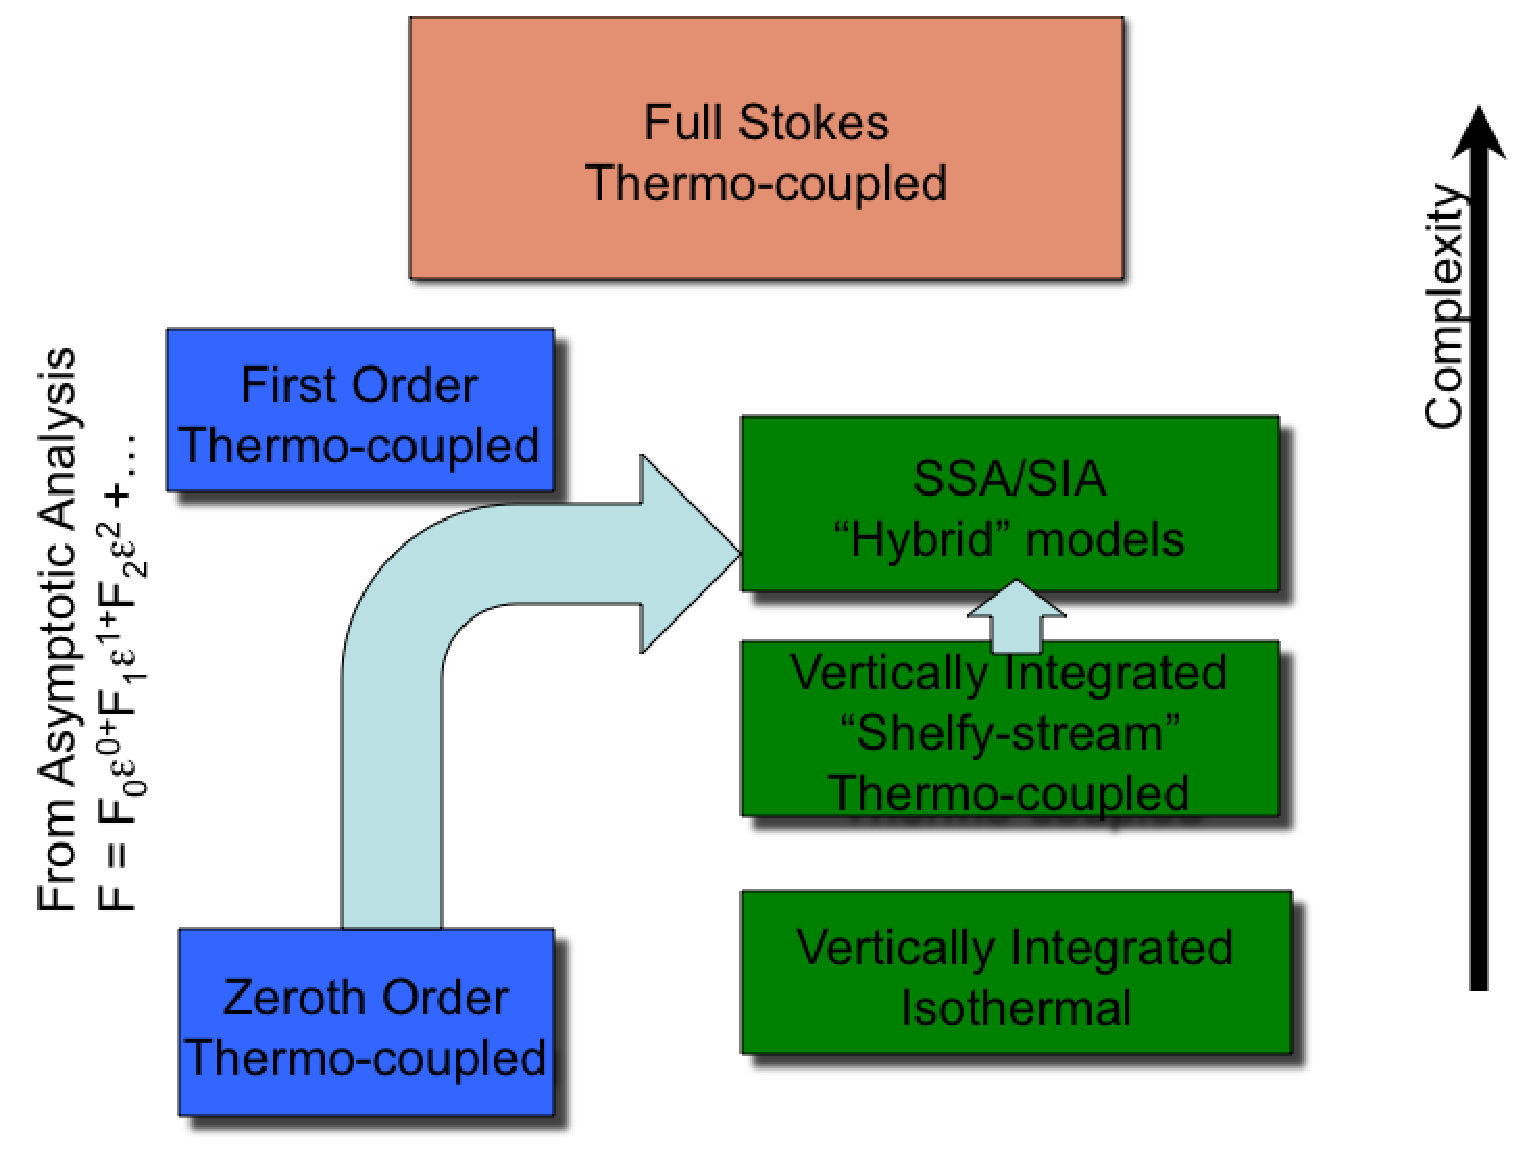
\includegraphics[width=0.5\columnwidth]{\dir/figs/ISMPhylogeny.eps}
   \end{center}
  \caption{The relationship between several common varieties of ice sheet modesl. Complexity increases along the vertical axis.}
   \label{fig:phylogeny}
\end{figure} 

There are large differences between shallow-ice and higher-order models in 
\textbf{(1)} how the momentum equations (the dynamics, or stress balance) are solved and 
\textbf{(2)} how the information derived from that solution (the kinematics, or velocity fields) is used to evolve the ice sheet geometry in time. There are two main reasons for these differences:

\begin{itemize}
\item  The numerical solution of the dynamical equations is fundamentally different. For the shallow-ice case, we need only local information (surface elevation and thickness) to solve for the velocity as a function of depth in a single column of ice. We do this pointwise for each location on the model domain (in map view), which is a relatively easy numerical problem.  Each column of velocities leads to a tridiagonal matrix that is easy to invert (i.e., to solve for the velocities). This problem is $embarrassingly$ $parallel$, since each column of unknown velocities results in a tridiagonal matrix that can be solved on a single processor. For higher-order models, however, the solution at any point also depends on the solution at neighboring points (in map view),
leading to an elliptic system of equations in which every velocity must be solved for simultaneously with every other velocity. The result is a much larger system of equations, which are more difficult to solve on one processor and far more difficult to solve on multiple processors. Because large-scale higher-order model applications (e.g., whole-ice-sheet models) require efficient, robust solution and parallelization techniques, this is an active area of current research.  
\end{itemize}

\begin{itemize}
\item  The equations governing dynamics AND evolution in a shallow-ice model can be recast as a nonlinear diffusion equation for ice thickness. A single system of equations is solved to calculate the velocity field and evolve the ice sheet geometry. For higher-order models, we must first solve the momentum balance equations to obtain the velocity field, and then use some other scheme to evolve the ice thickness. 
\end{itemize}

These differences imply that a higher-order model must be built in a fundamentally different way than a shallow-ice model.
Most recent development work on CISM has focused on higher-order dynamics.

%The equations describing a (2d) higher-order flow that is vertically integrated (i.e., the SSA) are:
%
%\begin{align*}
%\frac{\partial}{\partial x}\left ( 2 \eta H 
%\left(2\frac{\partial u}{\partial x}+\frac{\partial v}{\partial y}\right)\right)
%+\frac{\partial}{\partial y}\left(\eta H\left(
%\frac{\partial u}{\partial y}+\frac{\partial v}{\partial x}\right)\right)
%=\rho_w gH \frac{\partial s}{\partial x}
%\end{align*}
%
%
%\begin{align*}
%\frac{\partial}{\partial y}\left ( 2 \eta H 
%\left(2\frac{\partial v}{\partial y}+\frac{\partial u}{\partial x}\right)\right)
%+\frac{\partial}{\partial x}\left(\eta H\left(
%\frac{\partial u}{\partial y}+\frac{\partial v}{\partial x}\right)\right)
%=\rho_w gH \frac{\partial s}{\partial y}
%\end{align*}

Using the constitutive law from the lower panel of Figure \ref{fig:hoeqns}, the equations describing 3D higher-order flow\footnote{Specifically, the first-order accurate Stokes approximation discussed above. These will be derived in more detail in Section \ref{sc:higher-order-mom}.} are:

\begin{equation}
  \begin{split}
  & x: \frac{\partial}{\partial x}\left ( 2 \eta  
\left(2\frac{\partial u}{\partial x}+\frac{\partial v}{\partial y}\right)\right)
+\frac{\partial}{\partial y}\left(\eta \left(
\frac{\partial u}{\partial y}+\frac{\partial v}{\partial x}\right)\right)
+\frac{\partial}{\partial z}\left(\eta \frac{\partial u}{\partial z}\right)
=\rho_i g \frac{\partial s}{\partial x}, \\
  & y: \frac{\partial}{\partial y}\left ( 2 \eta 
\left(2\frac{\partial v}{\partial y}+\frac{\partial u}{\partial x}\right)\right)
+\frac{\partial}{\partial x}\left(\eta \left(
\frac{\partial u}{\partial y}+\frac{\partial v}{\partial x}\right)\right)
+\frac{\partial}{\partial z}\left(\eta \frac{\partial v}{\partial z}\right)
=\rho_i g \frac{\partial s}{\partial y}. \\
  \end{split}
\end{equation}


In these equations we can point out several important differences between shallow-ice and higher-order models: 
\begin{enumerate}
%\item  The vertically integrated model includes the ice thickness, $H$, in each term. This is a reflection of the integration and does not appear in the first-order equations.
%\item  Accounting for the thickness not appearing, the only other difference is the presence of a vertical diffusion of horizontal velocities. This is the the third term on the left in the above equations.
\item  The third term on the left-hand side represents the vertical diffusion of horizontal velocities. In a shallow-ice model, this term alone accounts for all ice dynamics and balances the entire body force in the $x$ direction (the term on the right-hand side). Since the velocity gradients are only in the vertical direction, the solution is local (in map view).

\item  The first-order equations must be solved for each of a set of horizontal layers (the number of which is defined by the resolution in the vertical, here $dz$). These layers communicate with each other through the vertical diffusion term.

\item  The first and second sets of terms on the left-hand side represent the resistance to the body-force term from ``membrane stresses" (i.e., stresses arising from horizontal velocity gradients). These horizontal gradients make the problem elliptic and non-local. The absence of membrane stresses in the shallow-ice momentum balance is the primary reason for their failure to realistically simulate the flow in outlet glaciers, ice streams, and ice shelves.

\end{enumerate}

%Both sets of equations are non-linear elliptical equations and much of the same technology can be used solve them. 
Other complications arise when we account for boundary conditions at the lateral margins of the domain and at the upper and lower ice surfaces. We describe both the governing equations and the boundary conditions in more detail below.
% (note that for the vertically integrated flow, there are no explicit boundary conditions for the upper and lower surfaces; they are accounted for and incorporated during the vertical integration).

%\subsection{Higher-order CISM}

%A very useful higher-order model intercomparison project (ISMIP-HOM) was organized by Frank Pattyn from the Université Libre de Bruxelles. That project, which resulted in a set of "benchmark" experiments for higher-order models, is reported on formally in Pattyn et al. (2008). 
